\chapter{Results}
\label{chap:results}
In this chapter the results of the experiments are presented. They are divided into three sections that were conducted consecutively to answer the research question that were posed in the introduction. The first section shows an analysis of the OES spectrum of the APP and confirms the plasma composition. The second section describes the effect of UV radiation had on the spores of C. sphaerospermum in the experiment. In the third section results of the APP treatment on the spores of C. sphaerospermum with and without reactive species are shown. 

\section{OES Analysis}
\label{sec:oes_analysis}
In the following the OES spectrum of the plasma first shown in section \ref{sec:oes} is analysed. To do so, the peaks of the spectrum are found using \textsc{Python} and the \textsc{SciPy} library. They are then compared to possible different species that could be present, and their wavelengths matched to identify the transitions. Figure \ref{fig:oes_analysis} shows the spectrum with the peaks marked using \cite{nist, spectra, spectrum}. The spectrum confirms the presence of the main species in the plasma, which are as expected mostly nitrogen, oxygen and water. Most oxygen is dissociated and makes new compounds with hydrogen or nitrogen leaving nitrogen molecules to be dominant in emission. Almost all visible peaks were found to correspond to the Second Positive System (2PS) of nitrogen. The 2PS is a system of transitions between the vibrational levels of the first excited state of nitrogen:
\begin{equation}
    \mathrm{N_2\ C^3\Pi_u \rightarrow B^3\Pi_g}
\end{equation}
and consists of many bands. Figure \ref{fig:n2_2ps} shows a plate of the 2PS of molecular nitrogen.


\begin{figure}
    \centering
    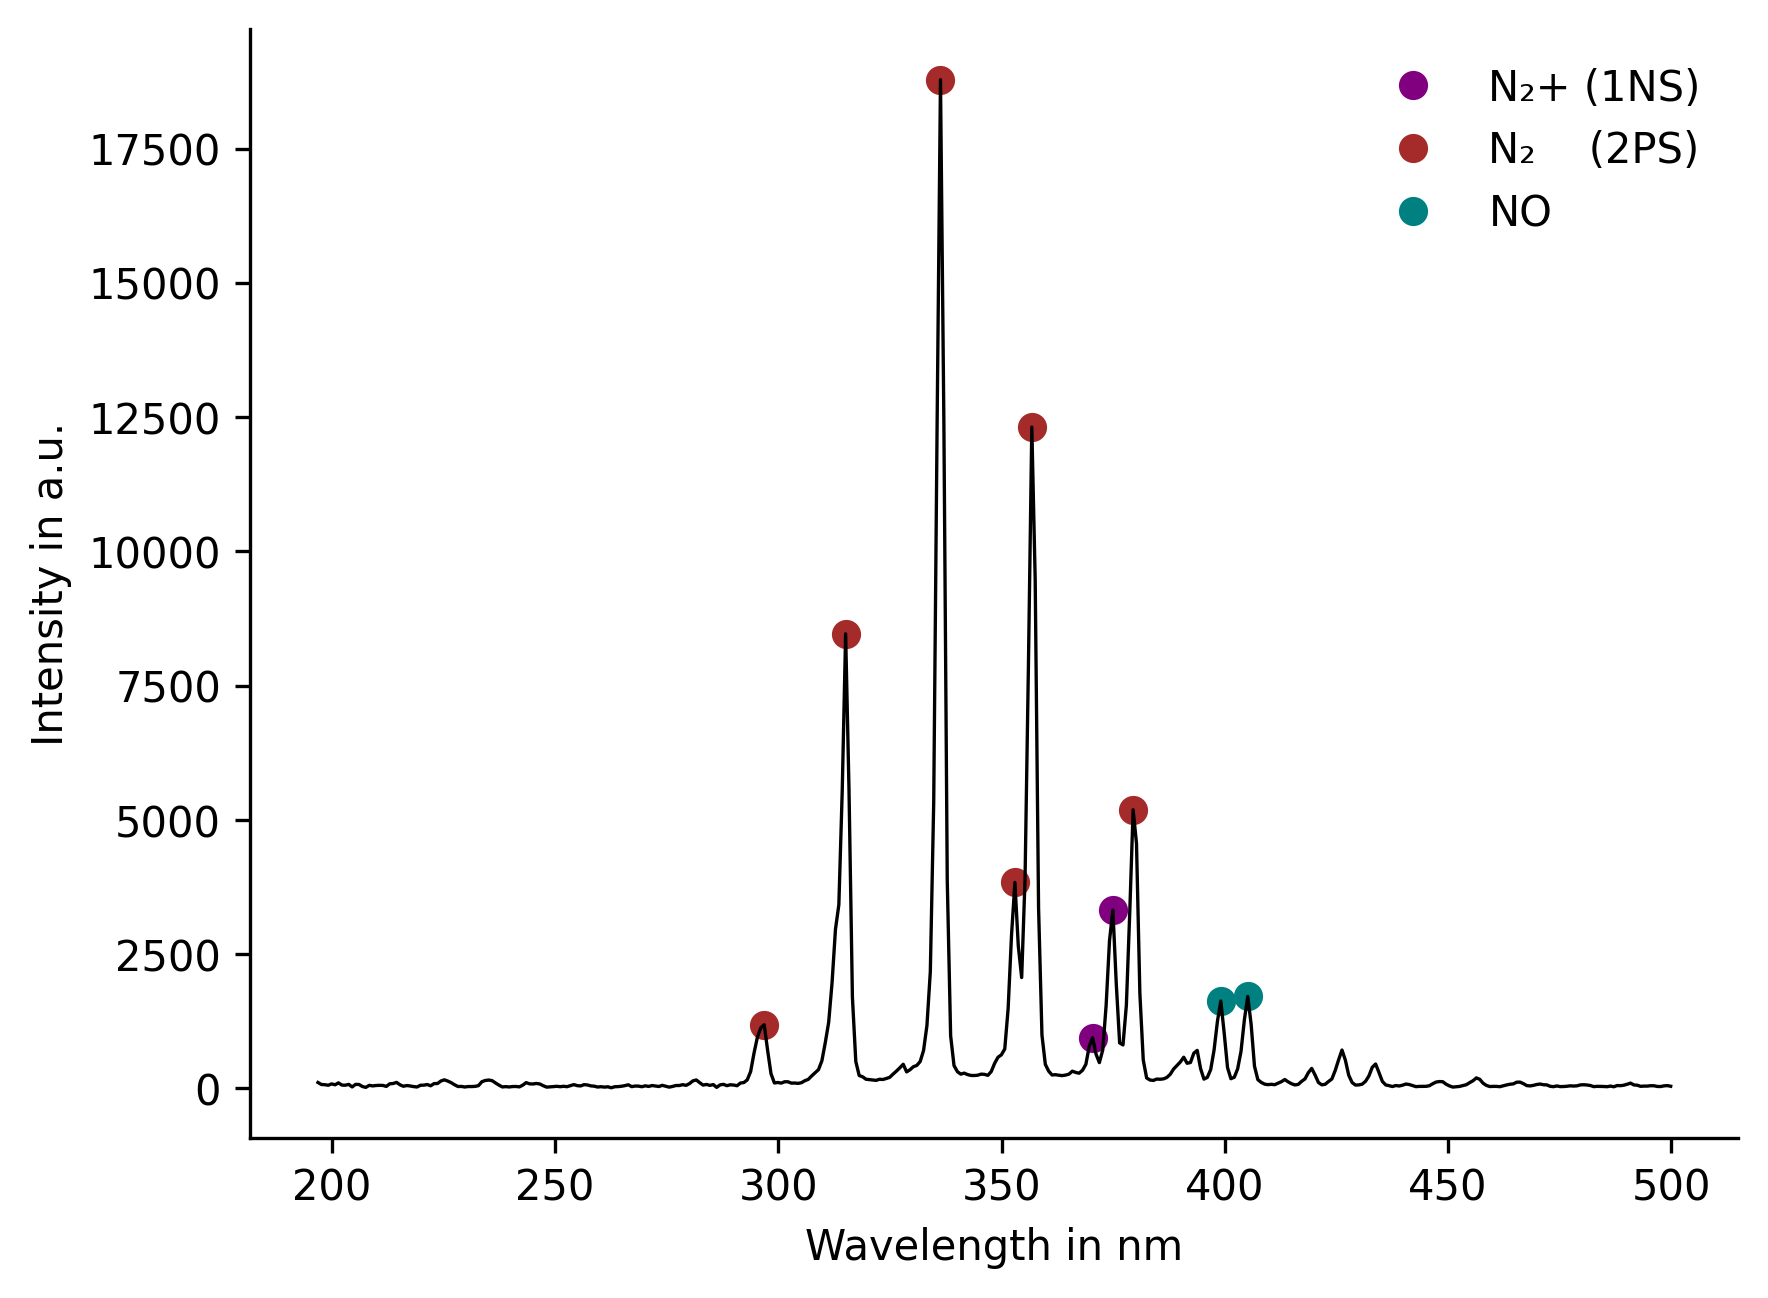
\includegraphics[width=1\textwidth]{images/OES_analysis.png}
    \caption[OES spectrum with identification]{OES spectrum of the plasma with the peaks identified. The Second Positive System of molecular nitrogen is dominant.}
    \label{fig:oes_analysis}
\end{figure}

\begin{figure}
    \centering
    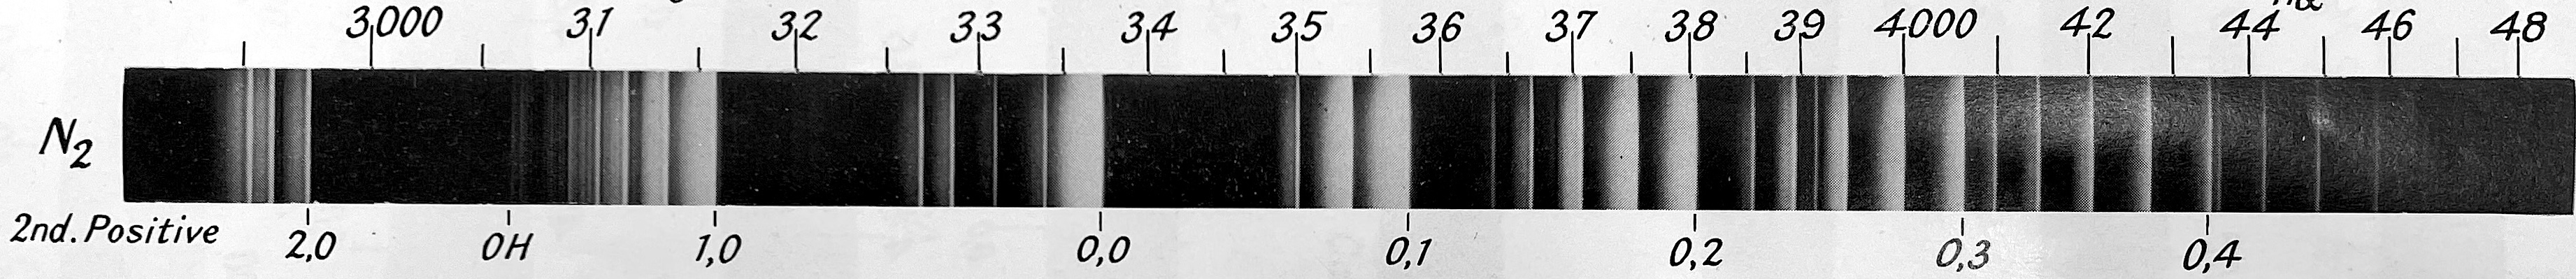
\includegraphics[width=1\textwidth]{images/N2_2PS.jpeg}
    \caption[Dinitrogen Second Positive System from literature]{Plate of the Dinitrogen Second Positive System from \cite{book}. The wavelengths are displayed above the photograph in Å.}
    \label{fig:n2_2ps}
\end{figure}


Using data from \cite{coefficients} listed in Table \ref{tab:boltzmann} (Appendix) and the OES spectrum of the plasma a Boltzmann plot is created. It is shown in Figure \ref{fig:boltzmann}. By calculating the slope of the plot from relative intensities the electron temperature can be estimated. As mentioned in \ref{sec:boltzmann} this can not be used as an absolute measurement in this work, because the plasma is non-thermal and is not in a local thermal equilibrium. From the slope obtained by fitting the data a temperature value of around 6500 K is found which appears to be in the expected order of magnitude. It lies between the values (3365 K -- 9168 K) that were found in \cite{oes_temperature} for an Argon plasma with a similar setup. This result also supports the correct identification of the observed emission peaks as transitions of the 2PS of molecular nitrogen.

\begin{figure}
    \centering
    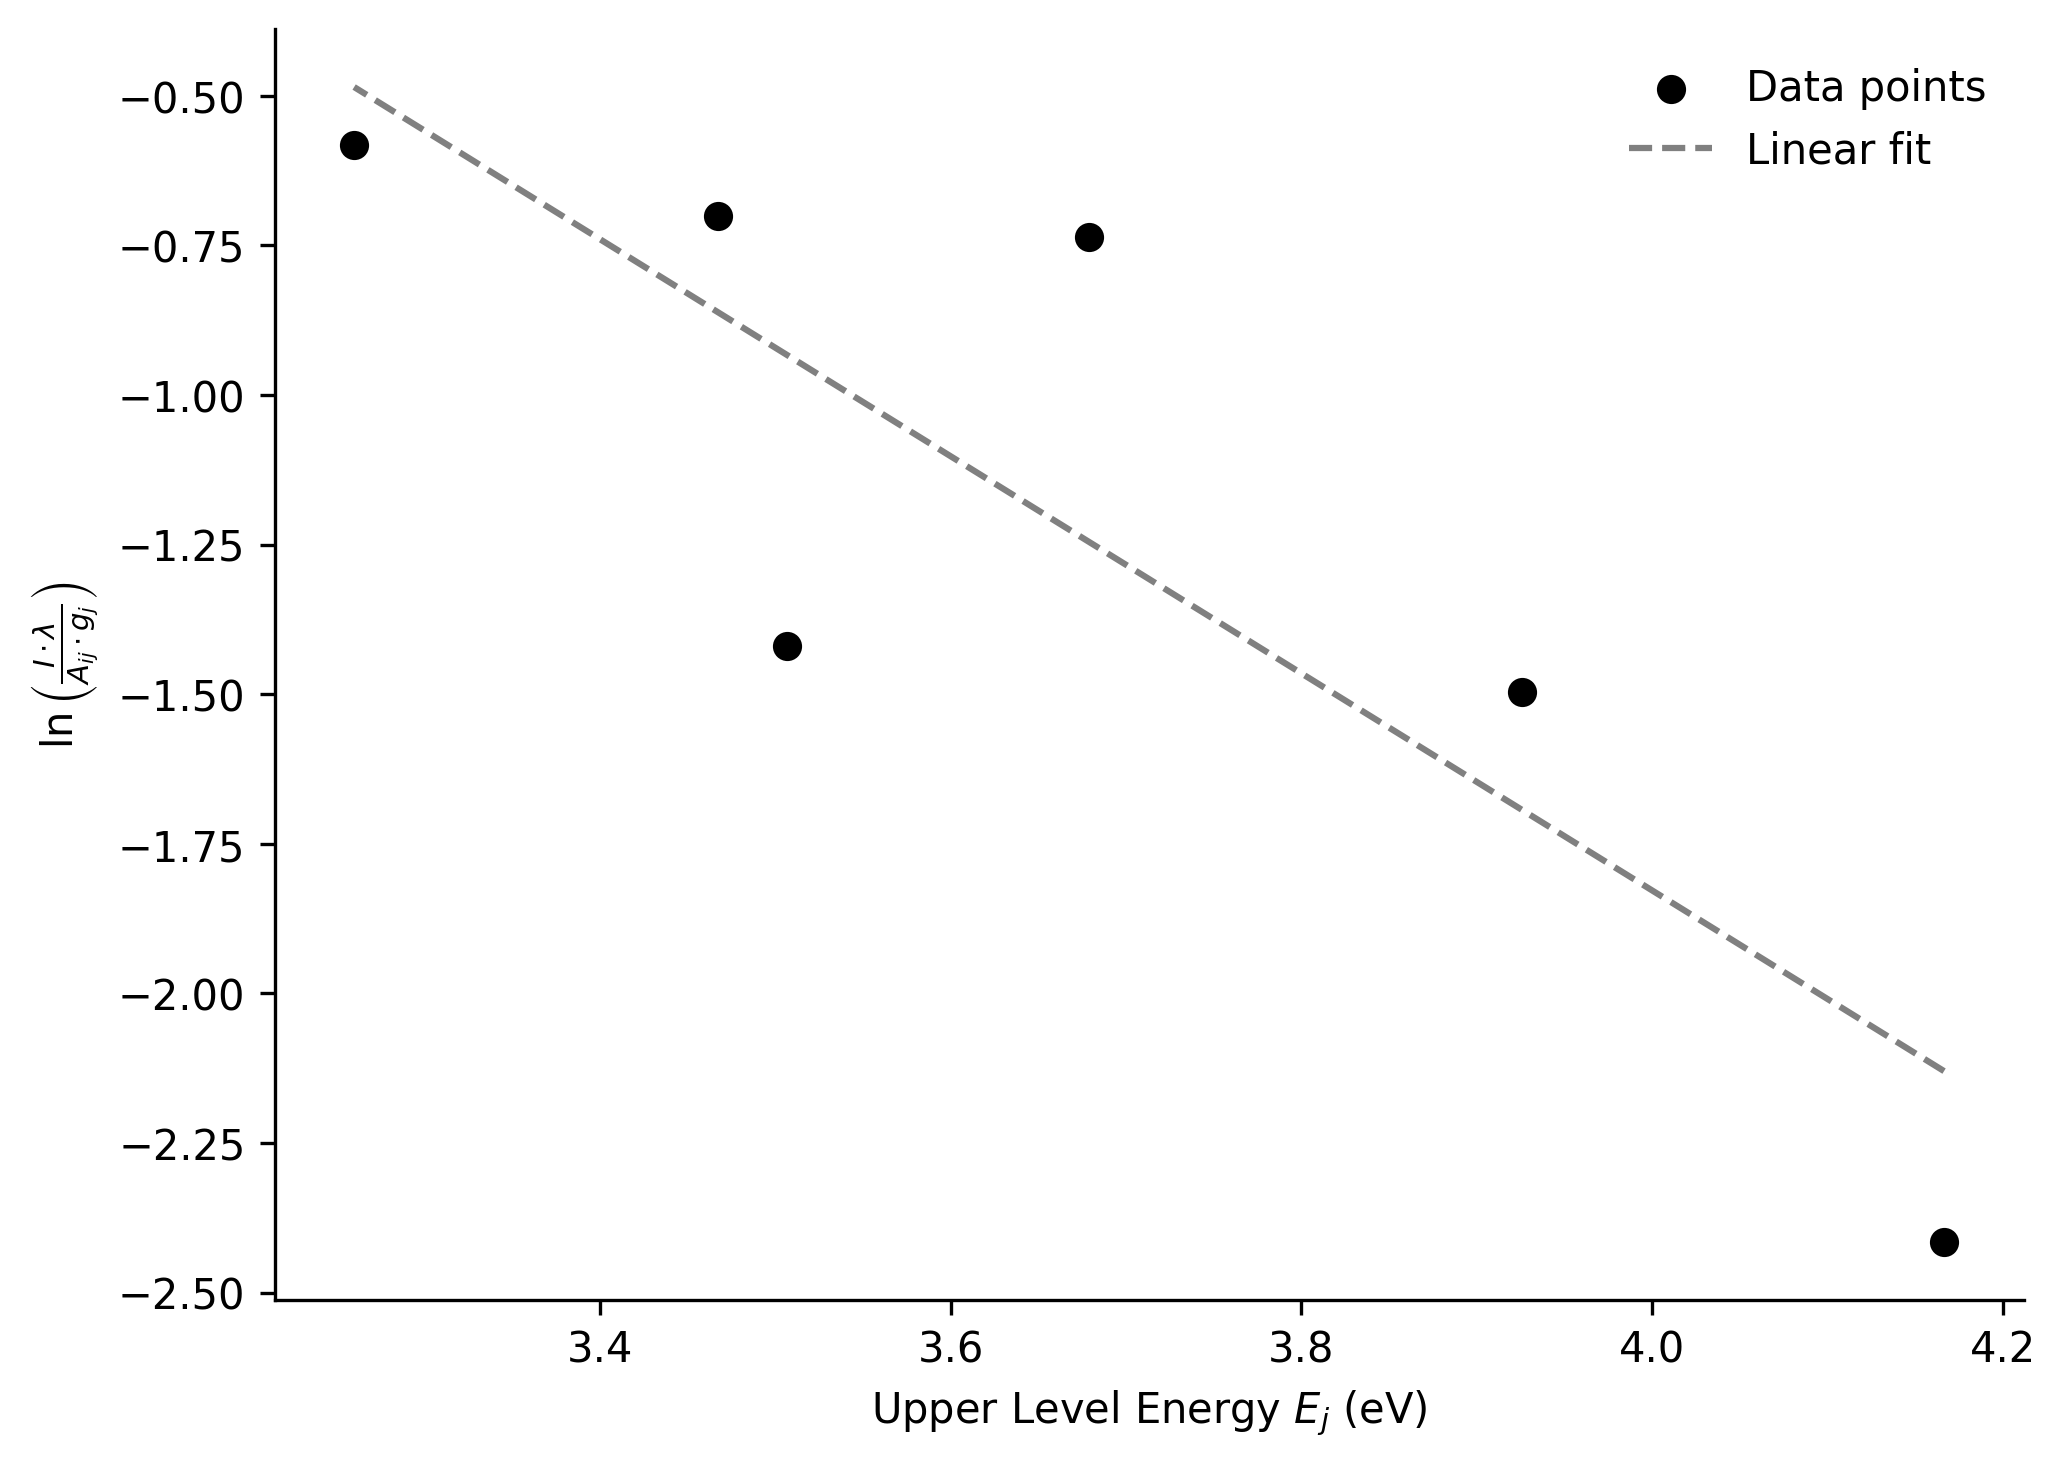
\includegraphics[width=.85\textwidth]{images/boltzmann_plot.png}
    \caption[Boltzmann Plot to estimate electron temperature]{Boltzmann Plot to estimate electron temperature using data from \cite{coefficients} listed in Table \ref{tab:boltzmann}.}
    \label{fig:boltzmann}
\end{figure}

\section{Effect of UV Exposure}
To confirm the effect of UV radiation on the spores of C. sphaerospermum, a control experiment is performed. First the spores are exposed to the UV lamp on agar medium for different times. After 15 min of exposure full deactivation was achieved. To control for the effect of the UV light on the agar medium, a second experiment is performed where the agar medium and spores are exposed to the UV light separately. To expose the spores they are instead put into the UV light in water and added to untreated agar media later. In Figure \ref{fig:uv_experiment} the petri dishes after incubation are shown. Table \ref{tab:uv_matrix} shows the number of colonies in a matrix. It becomes clear from this data that the UV light has no significant effect on the agar medium while it has a strong effect on the spores after an exposure time of 15 minutes. Using equation \ref{eq:uv_dose} the dose of UV radiation can be estimated and equates to 1.03 mJ/cm$^2$.

\begin{figure}
    \centering
    \begin{subfigure}[b]{0.6\textwidth}
        \centering
        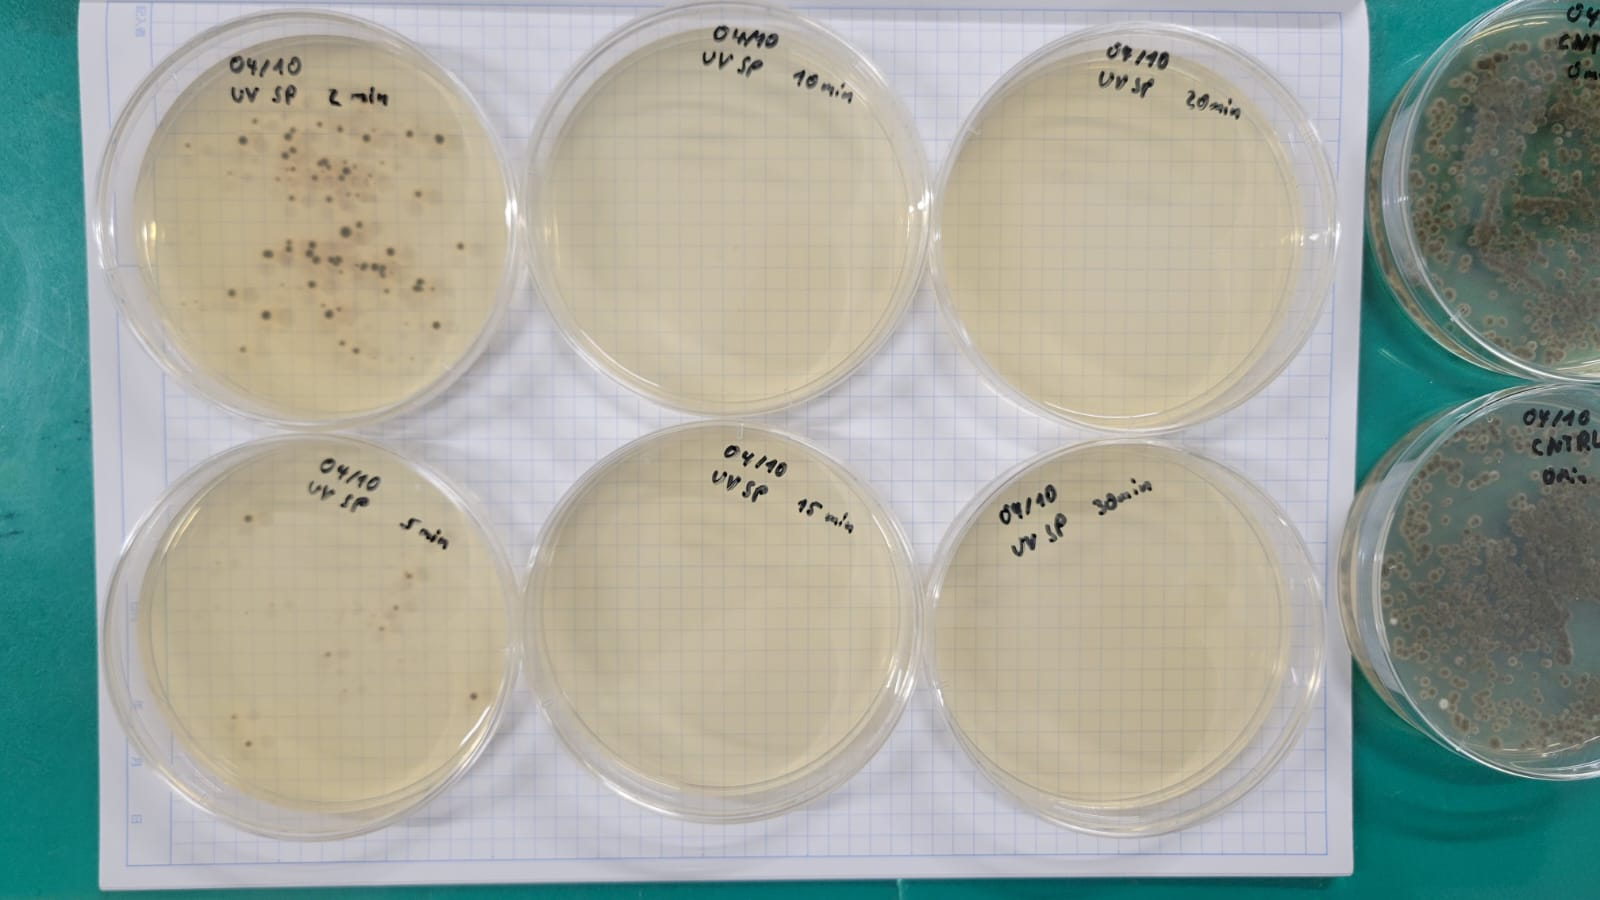
\includegraphics[width=\textwidth]{images/UV_SP.jpeg}
        \caption{Spore UV exposure}
        \label{fig:uv_a}
    \end{subfigure}
    \vfill
    \begin{subfigure}[b]{0.6\textwidth}
        \centering
        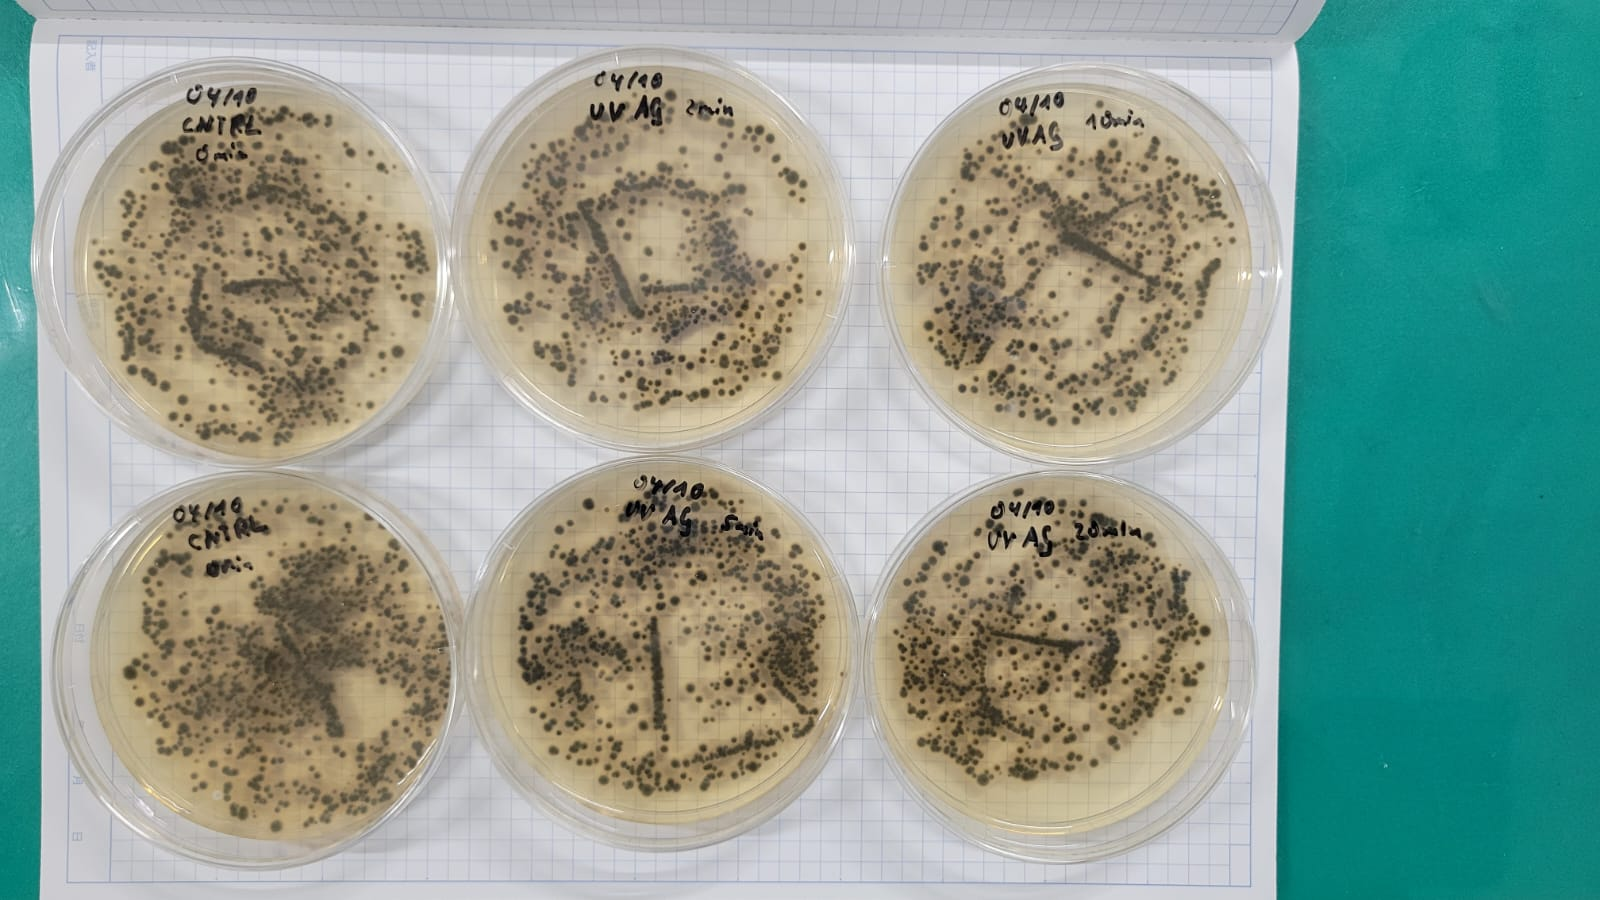
\includegraphics[width=\textwidth]{images/UV_AG.jpeg}
        \caption{Agar UV exposure}
        \label{fig:uv_b}
    \end{subfigure}
    \caption[Photograph of Petri dishes after treatment]{Petri dishes with spores (a) and agar (b) treated with UV light}
    \label{fig:uv_experiment}
\end{figure}

\begin{table}
    \centering
    \caption[Number of colonies after UV exposure as a matrix]{Number of colonies after UV exposure as a matrix. The results after 15 minutes are shown with an estimated dose of ca. 1.03 mJ/cm$^2$.}
    \vspace*{1em}
    \renewcommand{\arraystretch}{1.4}
    \setlength{\tabcolsep}{12pt}
    \begin{tabular}{c|cc}
        {\# of colonies} & {Spores no UV} & {Spores UV} \\
        \hline
        Agar no UV & >100 (cntrl) & 0 \\
        Agar UV    & >100 & 0 \\
    \end{tabular}
    \label{tab:uv_matrix}
\end{table}


\section{Effect of Plasma Treatment}